\BiChapter{实验测试与分析}{}

\BiSection{实验设置}{Subequations}
\BiSubsection{数据集与评价指标}{}



我们在流行的对话数据集DailyDialog \cite{li2017dailydialog}上进行实验。
DailyDialog 数据集是一个基于英语的自然人类交流数据集,由 13,118 个对话构成,共计 243,342 句话语。每个对话都具有一个主题,并由多个参与者共同完成,涵盖了我们日常生活中的各种话题。所有的话语都被贴上了情绪类别的标签,包括愤怒、厌恶、恐惧、高兴、中性、悲伤和惊讶。 图\ref{fig:dataset1} 和
% \ref{fig:dataset2}
4.1.2
中绘制了 DailyDialog数据集中情感和话题的分布情况。
DailyDialog 数据集中的情感标注是通过将情感标签与每个话语相关联的方式完成的。具体而言,每个话语都被标记为一个或多个情感类别。在标注中,情感标签不仅考虑了话语背后的主观情感体验,还考虑了话语所传递的语义、语境等因素。


\begin{figure}[ht] \label{decom}
    \vspace{15pt}

    \centering
 % \subfigure[Symmetric noise.]
 \hspace{-0.2cm}
 {
    \begin{minipage}{0.48\linewidth}
    \centering  %图片全局居中
    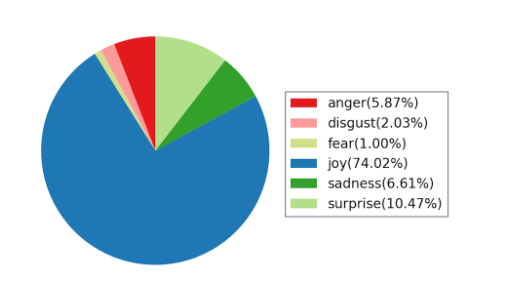
\includegraphics[width=\linewidth]{figures/dataset1.png}
    \label{fig:dataset1}
    \caption{DailyDailog数据集中的情感分布。}
    \end{minipage}}
 {
    \begin{minipage}{0.48\linewidth}
    \centering  %图片全局居中
    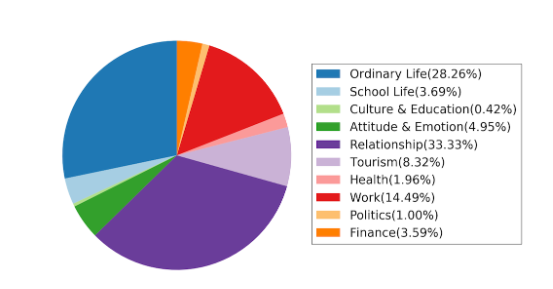
\includegraphics[width=\linewidth]{figures/dataset2.png}
    \label{fig:dataset2}
    \caption{DailyDailog数据集中的话题分布。}
    \end{minipage}}
    \vspace{10pt}
\end{figure}
    


研究者\cite{reccon}针对ECPE任务进一步对其进行了情感原因标注,形成了RECCON-DD 数据集。在 RECCON-DD 中,情感原因是通过标注者对每个话语所表达的情感进行分析完成的。标注者确定了每个话语表达的情感类型,以及产生该情感的具体原因或引发情感的事件、对象或事物等。标注者在标注情感原因时,着重考虑了上下文和对话的历史背景信息,以更好地理解和识别情感的来源和产生原因。
 RECCON-DD 中使用多个层面的标注者一致性指标来评估情感原因标注的准确性和一致性。同时,标注者在标注之前需要接受详细的指导和培训,以确保他们能够准确地理解和应用标注指南。这种方式可以帮助保证 RECCON-DD 数据集中情感原因标注的高质量和一致性。RECCON-DD 中的情感标注偏向于中性,其中 83\% 的话语被标记为中性情感,是一个适合用于情感原因识别任务的数据集,在不同于其他现有对话数据集上,更加贴近自然人类交流的情形。


我们使用以下评估指标:
\textbf{$F1_{Pos}$}: 这是由研究者\cite{rajpurkar2016squad} 提出的 F1 分数,用于评估抽取式 QA 模型的预测结果,并在数据中计算正例的 F1 分数。
\textbf{$F1_{Neg}$}: 负例 F1 表示相对于标准数据检测负例的 F1 分数。
\textbf{$F1_{macro}$}: 对每个正例和负例都计算 $F1$ 分数,然后对它们求平均。
此外,在消融实验中,为了更好的探究模型的性能变化,我们仅使用宏观$F1$值,还使用精确率(Precision, P),召回率 (Recall, R)作为额外的评价指标。P, R, F1 的计算公式如下:

\begin{equation}
\begin{aligned}
P = & \frac{TP}{TP+FP} \\
R = & \frac{TP}{TP+FN} \\
F1 = & 2 \times \frac{P \times R}{P+R}
\end{aligned}
\end{equation}
\vspace{6pt}

其中,TP 表示真阳性(即模型将正例正确地预测为正例的数量),FP 表示假阳性(即模型将负例错误地预测为正例的数量),FN 表示假阴性(即模型将正例错误地预测为负例的数量)。
F1 分数可以衡量模型在精度和召回率之间的平衡。在实际应用中,我们通常希望同时最大化 P 和 R 的值,因为这表示模型能够在较高的精确率下检测到更多的正例。


\BiSubsection{基线方法}{}

我们将我们的模型与几组知名的先进方法进行了比较。我们将它们详细说明如下:

\textbf{Inter-EC}。由研究人员\cite{DBLP:conf/acl/XiaD19} 提出的一个两步方法首先分别提取情感和原因。然后,为了形成ECP,它训练了一个二元分类器来过滤ECP和非-ECP。

\textbf{RankCP}。一种基于GAT的方法\cite{wei-etal-2020-effective}从排名的角度解决ECP预测问题,采用图注意力网络在子句之间传递信息。

\textbf{ECPE-2D}。一种基于Transformer的方法\cite{DBLP:conf/acl/DingXY20},用于构建一对矩阵,并通过利用2D transformer模块实现ECP之间的交互。

\textbf{MNLI}: 在MNLI上进行微调的RoBERTa: Roberta模型已在Multi-NLI数据集\cite{kim2019semantic}上进行了微调,并在句子对分类任务(例如自然语言推理)中展示了令人印象深刻的性能。我们将此方式作为我们的另一基准。

\BiSubsection{实验环境与细节}{}

我们使用RoBERTa - Base模型,并在隐藏状态输出上添加一个线性层来计算跨度开始和结束对数。
按照惯例,预训练语言模型首先在训练 Dag-Rank 时冻结其参数。我们采用 RoBERTa-Base \cite{liu2019roberta} 作为特征提取器,具有相同的体系结构。具体来说,对于每个话语 $c_i$,我们在其标记前添加一个特殊的标记   $[CLS]$,使输入形式为 $\{[CLS],w_{i1}, w_{i2},...,w_{in_i}\}$。然后,我们使用最后一层的 $[CLS]$ 汇聚嵌入作为 $c_i$ 的特征表示。
对于在 \ref{sec:build_dag} 中介绍的 $\omega$ ,我们默认将 $\omega=1$ 用于整体性能比较,但我们在 \ref{sec:layers} 中报告了  $\omega$ 从 1 到 3 不同取值的结果。我们将在 \ref{sec:loss} 中介绍的主损失函数设置为二分类交叉熵。
% $\beta$ 设置为$0.2$,将
所有隐藏向量的大小都为 300,RoBERTa 提取器的特征大小为 1024。
每个训练和测试过程都在单个 RTX 3090 GPU 上运行。搜索的超参数包括学习率、批大小、dropout率。每个训练过程包含 30 个迭代。 我们实现的模型报告的结果都是基于验证集上$3$次随机运行的平均分数。


\BiSection{主要结果与分析}{Subequations}


\begin{table}[t]
\vspace{15pt}
\renewcommand{\arraystretch}{1.2}
\centering\wuhao
\caption{该表汇报了在RECCON数据集上情感-原因对提取的实验结果。}
     \vspace{3mm}
 {
 \begin{tabularx}{\textwidth} { 
   >{\centering\arraybackslash}X 
   >{\centering\arraybackslash}X
   >{\centering\arraybackslash}X
   >{\centering\arraybackslash}X }

   % {@{}lllcccc@{}}
    \toprule[1.5pt]
      \textbf{Model} & $F1_{Pos}$ & $F1_{Neg}$ & $F1_{macro}$ \\
    \midrule[1pt]
   ECPE-MLL    &  &  &   \\
    ECPE-2D   &  &  &   \\
    RankCP    &  &  &   \\
    MNLI   &  &  &  \\
    \underline{Dag-Rank (Ours)}   &  &  &   \\
    \bottomrule
   \end{tabularx}}

  \label{tab:res}
  \vspace{10pt}
\end{table}


在表格 \ref{tab:res} 中,我们展示了在RECCON数据集上的情感-原因对提取的实验结果。我们将我们的模型与一些已有的模型进行了比较,这些模型包括ECPE-MLL, ECPE-2D, RankCP, 以及 MNLI,基线的性能报告源于文章\cite{reccon}。结果表明,我们的模型在各项指标上都取得了相当优秀的结果。

我们可以注意到在负面情绪的F1得分上,我们的模型取得了$00.00\%$的高分,这是所有模型中最高的。这一结果彰显了我们模型在准确识别和提取负面情绪原因对方面的出色能力。
另外,我们的模型在宏观F1得分上也取得了最高的$00.00\%$,超过了其他所有比较模型。这一结果揭示了我们模型在整体性能上的优越性。它代表了模型在处理正面和负面情绪的情感-原因对任务上找到了良好的平衡,并在整体性能上胜过了其他所有模型。
虽然我们的模型在正面情绪的F1得分上并未领先,但是$00.00\%$的得分仍表明了我们模型在处理正面情绪的情感-原因对任务上具备优秀的能力。
更值得注意的是,尽管ECPE-2D在正面情绪的F1得分上略微超过了我们的模型,但在负面情绪的F1得分和宏观F1得分上,我们的模型仍然展现了显著的优势。这再次证实了我们模型在情感-原因对提取任务上的全面性能优越性。

总而言之,我们的一步方法  DAG-RANK  在多个任务上均表现出色,并且在提取情感-原因对、情感子句和原因子句方面优于其他基线系统。通过对多个对的提取和在不同子集上的比较,我们的模型在各方面都取得了显著的进步。与其他现有方法相比,我们的方法在提取正确的情感-原因对方面具有更高的召回率和相近的精确度,表明我们的一步方法在情感原因提取任务上具有很大的潜力。
表\ref{tab:display}内展示了一段完整长对话的情感原因对识别效果。


\begin{table}[t]
	\renewcommand{\arraystretch}{1.2}
	\centering\wuhao
   \caption{Dag-Rank方法在一段长对话文本下的部分结果展示,其中 || 为分隔每个子句的分隔符,可以看到我们方法具有良好的表现,能够充分挖掘对话文本内的情感与原因。}
   \label{tab:display}
   \vspace{4mm}
   \begin{tabularx}{\textwidth}{m{2cm}p{12.8cm}}
   \toprule[1.5pt]
   % \multicolumn{2}{c}{\vspace{2pt} \centering \textbf{Dag-Rank在一段长对话上情感原因对识别效果示例}\vspace{2pt}  } \\ \midrule[1pt]
      
   \centering \textbf{数据文本}  & Wow , there are so many lanterns to appreciate . Now , I can see why it's called the Lantern Festival . It deserves its name . || Yeah . People always enjoy the lighted lanterns and the gala performances . || What are they doing over there ? People keep on gathering there . || Did you notice the characters on the lanterns ? || Sure . But you know that I can't read any Chinese characters . What do they say ? || They are puzzles . It's a tradition to solve the puzzles on the lanterns during the Lantern Festival . || Very interesting . But I'm afraid we'd better do something else . Hey , look ! There is a huge lantern there . Let's get close to it . || It's really eye-catching . It's the biggest dragon lantern I've ever seen in all my life . || Really ? Then I'm really lucky . Oh , it's spewing fireworks from its huge mouth . || Very impressive . It's made of glass which makes it even brighter . || There are many Chinese characters on its body , too . What are they about ? Puzzles ? || Let me have a look . Oh , no . They are Chinese poems which describe this happy scene .
   \\     \midrule[1pt]
   \centering 真实标签   &    [1, 1] , [2, 1] , [2, 2] , [7, 2] , [7, 7] , [9, 8] , [9, 9] , [10, 9] , [10, 10] , [12, 11] , [12, 12]   \\  
   \centering 模型预测   &    [9, 9] , [10, 10] , [8, 8] , [2, 2] , [10, 9] , [9, 8] , [8, 7] , [7, 7] , [2, 1] , [10, 8] , [12, 11] , [9, 7] , [1, 1]     \\     \bottomrule
   \end{tabularx}
   
    \vspace{8pt}

   \vspace{10pt}
\end{table}



\BiSection{消融实验}{Subequations}


为了全面评估我们提出模型各组件对其性能的影响,并深入理解模型行为,我们需要明确哪些组件在模型中起到了关键作用,哪些则是辅助性的。为此,我们设计了一系列的消融实验,通过刻意省略某些组件,评估这些组件对模型输出的具体贡献。以下内容会对我们进行的一些关键实验进行详细的描述和分析。通过这些消融实验,我们对模型中各个组件的重要性有了深入的理解,为模型的进一步优化和改进提供了有益的启示。


\BiSubsection{低级任务监督信号}{}

我们的模型除了使用情感原因对提取的损失函数$\mathcal{L}_{\text{pair}}$作为监督信号,还使用了 $ \mathcal{L}_{\text{emo}} + \mathcal{L}_{\text{cau}}$作为低级监督信号用于子句对表示学习和排序。
为了验证低级监督的效果,我们仅使用$\mathcal{L}_{\text{pair}}$训练模型,将结果与我们完整模型的结果进行比较。


\begin{table}[ht]
   \vspace{8pt}
   \renewcommand{\arraystretch}{1.2}
   \centering\wuhao
   \caption{不同层次任务监督信号的测试结果。}
    \label{tab:subloss}
   
   \vspace{4mm}
    
    \begin{tabularx}{\textwidth} { 
      >{\centering\arraybackslash}X 
      >{\centering\arraybackslash}X
      >{\centering\arraybackslash}X
      >{\centering\arraybackslash}X 
   }

   \toprule[1.5pt]
\textbf{损失函数}             & 精确率 & 召回率 & F1值 \\     \midrule[1pt]
w/ ( $\mathcal{L}_{emo} + \mathcal{L}_{cau}$ )    &  &  &  
    \\ 
w/o ( $\mathcal{L}_{emo} + \mathcal{L}_{cau}$ )     &  &  &     \\
w/o ( $\mathcal{L}_{emo} $ )         &  &  &    \\
w/o ( $\mathcal{L}_{cau}$ )         &  &  &    \\     \bottomrule
\end{tabularx}
\vspace{8pt}
\end{table}

我们将结果列举在表\ref{tab:subloss}中。结果表明,使用双层监督提高了提取性能。我们提供更丰富的监督信息,通过引入低级任务,我们为模型提供了更多的监督信息,使得模型可以从更多的角度理解和学习数据。低级任务的损失函数可以引导模型在学习主任务的同时,也关注到情感和原因子句的识别和分类。这种多任务学习的方式,可以促使模型在学习过程中更好地平衡各种任务,从而提高模型的泛化能力和预测性能\upcite{Li2020MultiTaskLW}。这将有助于模型更好地理解和区分情感子句和原因子句,从而更准确地提取出情感-原因对。


\BiSubsection{图神经网络结构}{sec:variants}

\textbf{局部连接影响: }
在本节中,我们通过将不同的 DAG 结构应用于 Dag-Rank,研究 DAG 的结构如何影响我们的 Dag-Rank 的性能。
除了我们提出的结构之外,我们还定义了三种 DAG 结构:
(1)序列,其中话语按顺序连接;
(2)最近局部信息,即具有单一局部信息的 DAG。在这种 DAG 中,每个话语仅从其最近邻居接收局部信息。
% ,而远程信息与我们的 DAG 相同;
(3)具有不同 $\omega$ 的 DAG,在这个 DAG 中,每个话语与之前的 $\omega$ 个话语相连。
我们在表 \ref{tab:variants} 中报告测试性能,以及每个话语的前驱节点的平均数量。

\begin{table}[ht]
   \vspace{8pt}
   \renewcommand{\arraystretch}{1.2}
   \centering\wuhao
   \caption{不同DAG结构的 Dag-Rank 模型测试结果。}
	\label{tab:variants}
   \vspace{4mm}
    
    \begin{tabularx}{\textwidth} { 
      >{\centering\arraybackslash}X 
      >{\centering\arraybackslash}X
      >{\centering\arraybackslash}X
      >{\centering\arraybackslash}X 
   }

        \toprule[1.5pt]
        \textbf{DAG结构}             & 精确率 & 召回率 & F1值 \\ \midrule[1pt]
        序列              &  &  &  \\
        最近局部信息    &  &  &     \\ 
        $\omega=1$          &  &  &    \\
        $\omega=2$         &  &  &     \\
        $\omega=3$         &  &  &     \\ \bottomrule
            
        \end{tabularx}

\vspace{10pt}
\end{table}

我们将这些不同的结构应用到Dag-Rank中,并比较了他们的性能。
从实验结果可以观察到几个有启发性的特点。首先,当应用序列结构时,结果F1值仅为$00.00\%$,表现较弱。当我们的Dag-Rank应用了单一局部信息的结构时,F1值提高到了$75.1\%$。而当我们将DAG结构应用到Dag-Rank时,F1值进一步提升,其中 $\omega=1$结构的F1值最高,达到了$00.00\%$。但是当 $\omega$ 继续增加,性能似乎略有下降。这表明,在我们的任务中,将每个话语与其最近的前驱连接可能是更有效的方法。
增加 $\omega$ 并没有显著提升性能,而且 $\omega=1$ 的情况下已经得到了相当好的结果,这可能有几个原因:当 $\omega$ 增大时,可能会引入更多的信息,但这些信息可能是冗余的,因为相近的话语往往具有相似的上下文。因此,增加更多的前驱节点并不能提供更多的新信息;此外,增大 $\omega$ 会导致更远的话语被引入为前驱节点。这些远离当前话语的话语可能和当前话语的关系较弱,引入它们可能会增加噪声,反而影响模型的性能。

这些实验结果实了我们的DAG结构对Dag-Rank性能的影响,并揭示了优化该性能的一种有效策略:将每个话语仅与其最近的前驱节点相连。这种策略通过直接关注每个话语的最直接上下文,提高了模型在理解和利用话语信息方面的效率和准确性。同时,这也表明,根据发言者身份和位置关系设定的约束是一种有效的归纳偏差,使得我们的DAG结构比固定连接每个话语与特定数量的前驱节点的方法更具优势。

\textbf{DAG层数影响: }
\label{sec:layers}
众所周知,堆叠过多的GNN层可能会因过度平滑而导致性能下降\upcite{kipf2016semi}。我们研究当堆叠许多DAG层时是否会发生同样的现象。
我们在实验中对比了我们使用的DAGGNN模型与GAT网络\cite{velivckovic2017graph},分别改变它们的层数从$1$至$8$层,并观察了它们在测试集上对情感原因对提取的性能变化。我们在图 \ref{fig:layernum1} 中绘制了测试结果。



\begin{figure}[ht] \label{decom}
    \centering
 \hspace{-0.2cm}
    \centering  %图片全局居中
    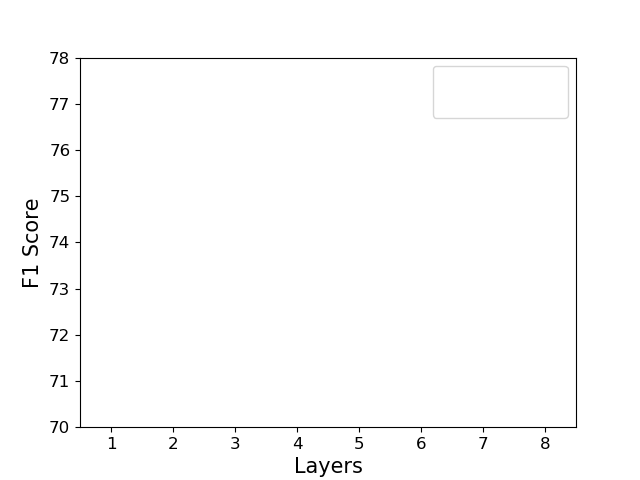
\includegraphics[width=0.6\linewidth]{figures/score.png}
    \label{fig:layernum1}
     \vspace{8pt}
    \caption{不同GNN层数对情感原因对提取的测试结果,横坐标为GNN层数,纵坐标为$F1$值。}
\end{figure}


    
实验结果显示,随着层数的增加,GAT的表现显著下降。这可能是由于堆叠过多的GNN层导致的过度平滑化现象,使得模型无法有效地捕捉和利用节点之间的复杂关系。这一结果与先前的研究结果相一致。
然而,对于DAGGNN模型,我们观察到一个有趣的现象。随着层数的增加,DAGGNN的性能在一个相对较窄的范围内波动,而没有出现显著的性能下降。这可能是因为在有向无环图网络中,每个节点的信息在传播过程中不会回到自身,从而避免了过度平滑化现象。

这些实验结果说明,在有向无环图网络中,我们可以通过增加层数来获取更远的节点信息,而不需要担心过度平滑化问题。这为我们在图神经网络设计和应用方面提供了有价值的指导。

\BiSubsection{相对位置嵌入}{}

在我们的实验中,我们研究了相对位置嵌入对情感原因对提取性能的影响。我们对比了以下三种不同的设置:
(1)不使用相对位置嵌入:我们将模型中的相对位置嵌入部分去掉,以验证其对模型性能的影响。
(2)普通相对位置嵌入:在这个设置中,我们使用传统的相对位置嵌入方案。
(3)核函数相对位置嵌入:我们采用基于核函数的相对位置嵌入方案,以考虑各个相对位置之间的相互影响。
实验结果如\ref{tab:embedding}所展示。


\begin{table}[h]
   \vspace{8pt}
   \renewcommand{\arraystretch}{1.2}
   \centering\wuhao
	\caption{不同种类相对位置嵌入方案的Dag-Rank测试结果。}
	\label{tab:embedding}
   \vspace{4mm}
    
    \begin{tabularx}{\textwidth} { 
      >{\centering\arraybackslash}X 
      >{\centering\arraybackslash}X
      >{\centering\arraybackslash}X
      >{\centering\arraybackslash}X 
   }

\toprule[1.5pt]
\textbf{相对位置嵌入方案}             & 精确率 & 召回率 & F1值 \\ \midrule[1pt]
None     &  &  &     \\
Vanilla    &  &  &    \\
Kernel     &  &  &    \\ \bottomrule
\end{tabularx}
\vspace{10pt}
\end{table}


首先,相对位置嵌入在情感-原因对提取任务中起着重要的作用。这可以从不使用相对位置嵌入和使用相对位置嵌入的实验结果对比中看出。不使用相对位置嵌入的情况下,模型的F1值为$00.00\%$,而在使用传统相对位置嵌入的情况下,F1值增加到$00.00\%$。这表明相对位置嵌入能够有效地捕捉和理解文本中的上下文关系,从而提高模型的性能。
其次,基于核函数的相对位置嵌入方案比传统相对位置嵌入方案更有效。传统相对位置嵌入方案的F1值为$00.00\%$,而使用基于核函数的相对位置嵌入方案,F1值进一步提升到$00.00\%$。这说明通过使用径向基函数(RBF)作为核函数来模拟不同相对位置之间的影响,能够更好地表示相对位置嵌入,从而进一步提升模型性能。

综上所述,考虑各个相对位置之间的相互作用有助于获得更强大的子句对表示,从而进一步提高情感原因对提取的性能。
相对位置嵌入在情感原因对提取任务中起到了关键作用,同时核函数相对位置嵌入相较于普通相对位置嵌入能够取得更好的性能。我们的消融实验对于如何利用位置信息来提升自然语言处理任务的性能提供了有益的见解。


\BiSubsection{排序方法比较}{}
我们评估了使用交叉熵损失函数$\mathcal{L}^{\text{ce}}_{\text{pair}}$与边界排序损失函数$\mathcal{L}^{\text{rank}}_{\text{pair}}$对模型进行训练的效果的影响。为了深入探索排序对我们模型的重要性,我们引入了一个系数$\lambda$,用于计算这两种损失函数的加权平均值作为最终的主损失函数,即$\mathcal{L}_{\text{pair}}=\lambda \mathcal{L}^{\text{rank}}_{\text{pair}} + (1-\lambda) \mathcal{L}^{\text{ce}}_{\text{pair}} $。相应的实验结果在表\ref{tab:rankingloss}中展示。


\begin{table}[ht]
   \vspace{8pt}
   \renewcommand{\arraystretch}{1.2}
   \centering\wuhao
	\caption{不同比例主损失函数的设置对性能的影响。}
	\label{tab:rankingloss}
   \vspace{4mm}
    
    \begin{tabularx}{\textwidth} { 
      >{\centering\arraybackslash}X 
      >{\centering\arraybackslash}X
      >{\centering\arraybackslash}X
      >{\centering\arraybackslash}X 
   }
\toprule[1.5pt]
\centering  \textbf{$\lambda$}   & 精确率 & 召回率 & F1值 \\ \midrule[1pt]
\centering 0     &  &  &      \\ 
\centering 0.25   &  &  &      \\
\centering 0.5   & & &     \\
\centering 0.75   &  & &        \\
\centering 1   &  &  &      \\ \bottomrule
\end{tabularx}
\vspace{10pt}
\end{table}


实验结果表明,进行对情感原因对进行交叉熵损失的效果略优于对所有样本对进行排序。
这可能是因为对情感原因对进行二分类判别有着更直接的优化目标,每个样本的得分都是独立计算和预测的,这种方法的优化目标更加直接明确,即两个子句是情感原因对的概率。
在大数据量情况下,二元或者更高阶的排序方法可能会引入更多的复杂性,因为他们要考虑样本之间的相对顺序。而进行直接优化相对简单,因为它只关注单个样本的预测。深度神经网络对于大数据量和高维度的数据具有很好的处理能力。在大数据量情况下,直接使用二分类优化可能相较于将候选的情感原因配对排序具有更好的效果\upcite{minaee2021deep}。

然而,将逐点方法(Pointwise)和成对方法(Pairwise)结合在一起,可以更好的提高模型的性能。这种混合方法能够同时考虑单个样本的得分和样本间的相对排序,在我们的场景下,比单独使用任何一种方法都要更好。这也说明排序损失函数的的合理性,证明在情感原因对筛选中应该考虑子句对之间的排序关系。
然而,需要注意的是,尽管这种混合方法可能在某些情况下效果更好,但它们也可能带来额外的复杂性,包括模型设计的复杂性和计算成本的增加。所以在实践中,是否使用混合方法,应根据具体任务的需求和资源限制来决定。


\begin{table}[ht]
   \vspace{15pt}
	\renewcommand{\arraystretch}{1.2}
	\centering\wuhao
   \caption{Dag-Rank方法在一段长对话文本下的部分结果展示,其中 || 为分隔每个子句的分隔符,可以看到如果包含原因和情感的子句距离过大,可能会影响图神经网络加强对话间子句特征的效果,从而影响情感原因溯源的能力。}
   \label{tab:error}
   \vspace{6mm}
   \begin{tabularx}{\textwidth}{m{2cm}|p{12.8cm}}
   \toprule[1.5pt]
   % \multicolumn{2}{c}{\vspace{2pt} \centering \textbf{Dag-Rank在一段长对话上情感原因对识别效果示例}\vspace{2pt}  } \\ \midrule[1pt]
      
   \centering \textbf{数据文本}  & I'm going to the store downtown this afternoon to try on my wedding dresses . || Oh my gosh , how exciting ! || Will you come with me and help me choose ? || Sure , I will . How can I miss that ? || Good . I think I'll get too nervous to look at myself in the mirror ! || Oh , don't . I'm sure you'll be the loveliest bride ever !
   \\     \midrule[1pt]
   \centering 真实标签   &   [1, 1] , [2, 1] , [2, 2] , [3, 1] , [3, 2] , [4, 1] , [4, 2] , [5, 1] , [5, 2] , [6, 1] , [6, 2] , [6, 6]  \\  \midrule[1pt]
   \centering 模型预测   &   [2, 2] , [1, 1] , [4, 2] ,[3, 1] , [4, 4] , [2, 1]    \\     \bottomrule
   \end{tabularx}
   \vspace{10pt}
\end{table}


\BiSection{误差分析}{Error Analysis}
在RECCON上进行情绪原因对提取任务实验时,我们发现了一些潜在的错误挑战。以下是我们的主要观察和分析:

    \textbf{情绪和原因的复杂性}:模型在理解和提取复杂情绪和对应原因的子句对时存在困难。例如,如果文本中的情绪和原因都有细微的差异,或者情绪和原因在文本中难以分开,那么模型可能无法准确提取。

    \textbf{隐含的原因}:有时候,导致某种情绪的原因并不是直接明显的。这些原因可能以隐含或者比喻的形式出现,或者是未在对话中明确提及的。在这些情况下,模型可能无法准确提取情感原因对。

    \textbf{上下文的重要性}:在一些情况下,理解情绪和原因需要对所有对话的上下文有深入的理解。如果上下文信息缺失或者模型没有充分理解上下文,那么就可能导致提取错误。如表\ref{tab:error}所展示,如果,目前的Dag-Rank模型可能会表现出不令人满意的效果。

    \textbf{情绪转移的挑战}:与我们在情绪识别任务中的发现类似,情绪转移对ECPE任务也是一个重大的挑战。当连续两个子句的情绪不一致时,模型可能会产生错误的情绪-原因对。

    \textbf{多种情绪的共存}:在有些情况下,一段对话可能表达了多种不同的情绪,并且每种情绪都有各自的原因。在这些复杂场景中,模型可能无法准确区分和提取每一对情绪-原因。

总的来说,虽然我们已经取得了一些进展,但我们的ECPE模型仍有很大的提升空间。以上是我们的主要观察,我们需要继续深入理解这些问题并设计更有效的解决策略,进一步提高文本情感溯源的能力。


\BiSection{本章小结}{expconclusion}

在该实验中,我们使用RECCON数据集评估了 Dag-Rank 的性能,并将其与其他模型进行了比较。结果表明,我们的模型在各项指标上都取得了相当优秀的结果。
通过消融实验,我们进一步评估了模型中各个组件的重要性,并深入理解了模型的行为。我们发现通过引入低级监督信号和使用多任务学习可以提高模型的性能,并在子句对表示学习和排序方面发挥作用。此外,我们还研究了DAG结构和层数对模型性能的影响,并发现将每个话语仅与其最近的前驱节点相连是一种有效的策略。最后,我们研究了相对位置嵌入对模型性能的影响,并发现基于核函数的相对位置嵌入方案比传统相对位置嵌入方案更有效。

综上所述,此章节展示的实验结果表明我们提出的模型在情感-原因对提取任务上取得了显著的进展,并且通过消融实验深入理解了模型中各个组件的作用。这些结果为进一步优化和改进我们的模型提供了有益的启示。